\documentclass[a4paper,12pt]{article}
\usepackage{cmap}
\usepackage[utf8]{inputenc}
\usepackage[english, russian]{babel}
\usepackage[left=2cm,right=1cm,top=2cm,bottom=2cm]{geometry}
\usepackage[pdftex]{graphicx}
\usepackage{hyperref}
\usepackage{wrapfig}
\graphicspath{{img/}}
\usepackage{float}

\begin{document}

\thispagestyle{empty}

\begin{figure}[h]
	\centering
	
\includegraphics[scale=0.60]{hudson-logo.png}
\end{figure}
\clearpage

\tableofcontents 
\clearpage

\section{Кратко о \href{http://hudson-ci.org/}{Hudson}}

Hudson - это Continuous integration сервер. Позволяет собирать
\href{}{Ant} и \href{}{Maven} проекты, которые могут быть выкачаны из разных
систем контроля версий. 

\subsection{Достоинства}
\begin{itemize}
  \item Распрастраняется под лицензией MIT
  \item Легок в освоении
\end{itemize}

\subsection{Требования}
Для работы Hudson должна быть установлена JDK.

\subsection{Уставновка}
Установка заключается в скачивании \texttt{war} файла с \href{http://hudson-ci.org/}{официального сайта}.

Дла запуска необходимо перейти в директорию с \texttt{war} файлом и выполнить команду 
`\texttt{java -jar <war-name>}` (`\texttt{war-name}` - заменить на имя скачанного War файла, 
например, для версии 2.2.0 - `\texttt{hudson-2.2.0.war}`)

После запуска можно открыть браузер и перейти на
\texttt{\href{http://localhost:8080/}{http://localhost:8080/}}. На
рис. \ref{pic.hudson.home} показана стартовая страница для версии \texttt{2.2.0}.

\begin{figure}[htp]
	\begin{center}
	  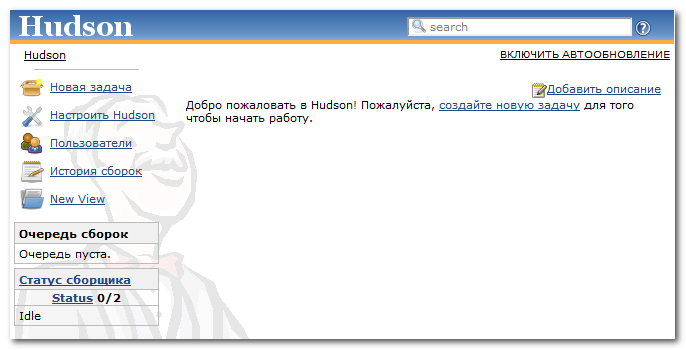
\includegraphics[scale = 1]{start.png}
	  \caption{Стартовая страница}
	  \label{pic.hudson.home}
	\end{center}
\end{figure}

\subsubsection{Настройка}

В качестве примера выполним настройку для сборки Maven проекта, который
находится в SVN-репозитории.

Для этого необходимо указать Hudson где находятся исполняемые файлы системы сбоки Maven. это можно сделать в подразделе
``\texttt{Конфигурирование системы}'' раздела  ``\texttt{Настройка Hudson}'' (см. рис. \ref{pic.hudson.configuration}, 
\ref{pic.hudson.configuration.system-options}, \ref{pic.hudson.configuration.system-options.maven}).

\begin{figure}[htp]
	\begin{minipage}[h]{1\linewidth}
		\begin{center}
			\begin{minipage}[h]{0.49\linewidth}
				\begin{center}
				  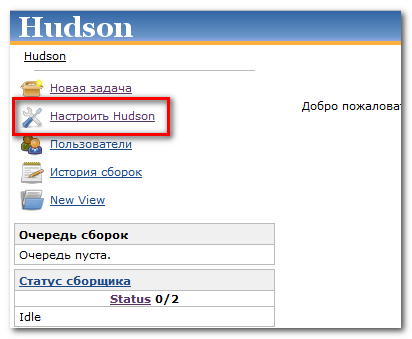
\includegraphics[scale = 0.8]{conf-1.png}
				  \caption{Стартовая страница}
				  \label{pic.hudson.configuration}
				\end{center}
			\end{minipage}
			\hfill
			\begin{minipage}[h]{0.49\linewidth}
				\begin{center}
					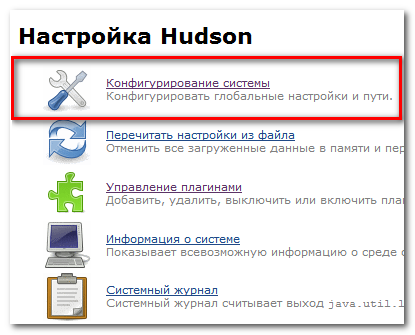
\includegraphics[scale = 0.8]{conf-2.png}
					\caption{Стартовая страница}
					\label{pic.hudson.configuration.system-options}
				\end{center}
			\end{minipage}
		\end{center}
	\end{minipage}
	\vfill
	\begin{minipage}[h]{1\linewidth}
		\begin{center}
			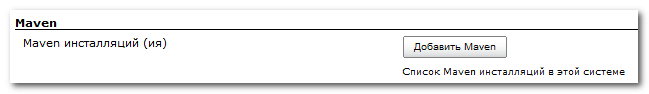
\includegraphics[scale = 1]{conf-maven.png}
			\caption{Стартовая страница}
			\label{pic.hudson.configuration.system-options.maven}
		\end{center}
	\end{minipage}
\end{figure}

В пункте ``\texttt{Maven}'' нужно нажать на кнопку ``\texttt{Добавить Maven}''. После этого появится новая инсталляция
Maven (см. рис. \ref{pic.hudson.configuration.system-options.maven-ni}). Если Maven уже установлен на сервере можно
убрать отметку с чекбокса ``\texttt{Install automatically}'' и укать путь в поле ``\texttt{MAVEN\_HOME}'' (см. рис.
\ref{pic.hudson.configuration.system-options.maven-conf}).

\begin{figure}[htp]
	\begin{center}
	  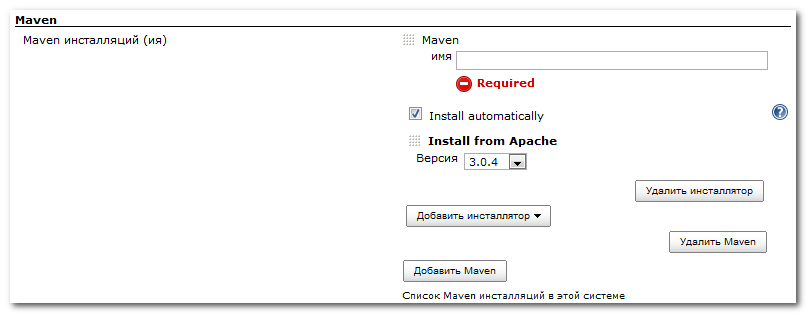
\includegraphics[scale = 0.6]{conf-maven-1.png}
	  \caption{Новая инсталяция Maven}
	  \label{pic.hudson.configuration.system-options.maven-ni}
	\end{center}
\end{figure}

\begin{figure}[htp]
	\begin{center}
	  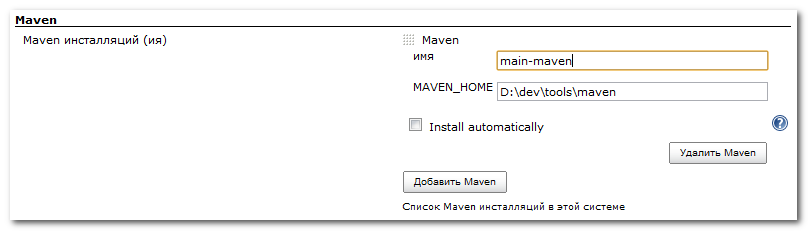
\includegraphics[scale = 0.6]{conf-maven-2.png}
	  \caption{Настройка Maven}
	  \label{pic.hudson.configuration.system-options.maven-conf}
	\end{center}
\end{figure}

Далее проведе конфигурацию SVN. Для этого в пункте ``\texttt{Subversion}'', на этой же странице, из выпадающего списка
``\texttt{Subversion Workspace Version}'' выберем ``\texttt{1.6 (svn:externals to file)}'' (см. рис.
\ref{pic.hudson.configuration.system-options.svn-conf}).

\begin{figure}[htp]
	\begin{center}
	  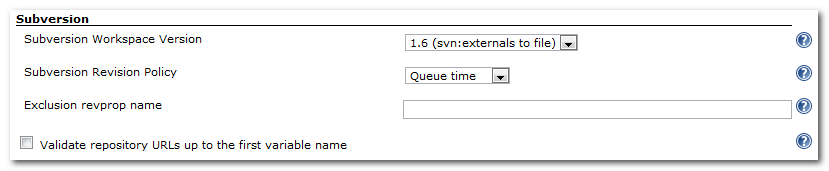
\includegraphics[scale = 0.6]{conf-svn.png}
	  \caption{Настройка Subverion}
	  \label{pic.hudson.configuration.system-options.svn-conf}
	\end{center}
\end{figure}

Настройка системы завершена. Сохранить измения можно с помощью кнопки ``\texttt{Сохранить}'' внизу страницы.

\subsection{Создание задачи} 
\label{sec.job-createion}
Для создания задачи (job) необходимо на боковой панели нажать на ссылку ``\texttt{Новая задача}'' (см. рис.
\ref{pic.hudson.sidebar.new-job}) в поле ``\texttt{Имя задачи}'' произвольное имя (например, имя проекта) и выбрать
``\texttt{Создать задачу со свободной конфигурацией}'' (см. рис. \ref{pic.hudson.sidebar.new-job}) и нажать на кнопку
``\texttt{OK}''.

\begin{figure}[htp]
\begin{center}
  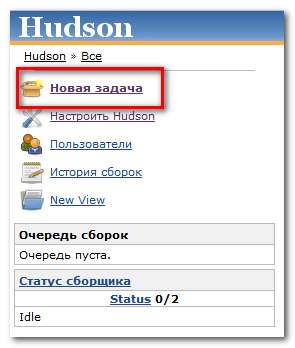
\includegraphics[scale = 0.6]{new-job-1.png}
  \caption{Боковая панель}
  \label{pic.hudson.sidebar.new-job}
\end{center}
\end{figure}

\begin{figure}[h!]
\begin{center}
  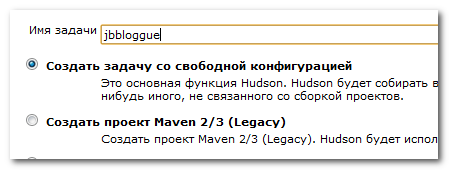
\includegraphics[scale = 0.8]{new-job-2.png}
  \vspace{-10pt}
  \caption{Создание новой задачи}
  \label{pic.hudson.job-creation}
\end{center}
\end{figure}

После этого загрузится страница конфигурирования задачи. На этой странице можно указать описание задачи и другий
параметры. Сейчас нам нужно указать что будет использоваться \texttt{SVN} в пункте ``\texttt{Управление исходным
кодом}'' (см.
рис.
\ref{pic.hudson.sidebar.new-job}). Далее в поле ``\texttt{URL репозитория}''указать путь к репозиторию, а из выпадающего
списка ``\texttt{Check-out Strategy}'' выбрать ``\texttt{Clean checkout folders and then checkout}''.

\begin{figure}[htp]
\begin{center}
  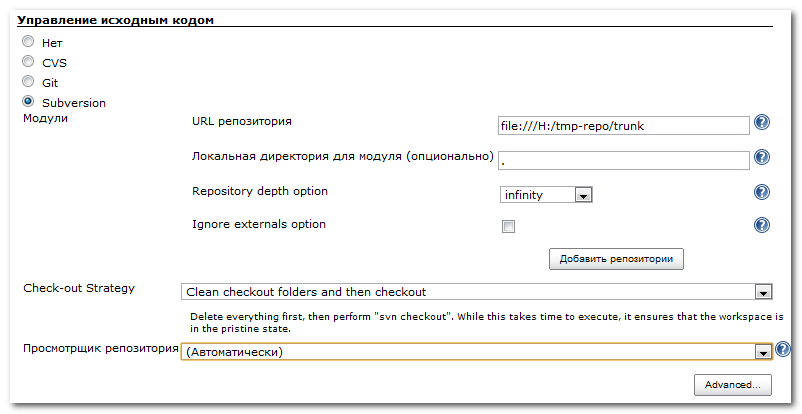
\includegraphics[scale = 0.8]{new-job-3.png}
  \caption[labelInTOC]{Конфигурирование SVN}
  \label{pic.hudson.job.svn}
\end{center}
\end{figure}

Далее в пункте ``\texttt{Триггеры сборки}'' отметить ``\texttt{Опрашивать SCM об изменениях}'' (см. рис.
\ref{pic.hudson.job.triggers}) и в появившемся поле ``\texttt{Расписание}'' указать ``\texttt{* * * * *}'' (проверять
каждую минуту).

\begin{figure}[htp]
\begin{center}
  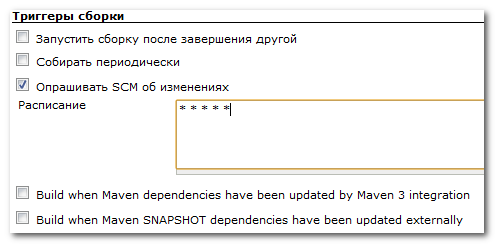
\includegraphics[scale = 0.8]{new-job-4.png}
  \caption{Триггеры сборки}
  \label{pic.hudson.job.triggers}
\end{center}
\end{figure}

В пункте ``\texttt{Сборка}'' укажем шаги сборки. Для этого нужно нажать на кнопку ``\texttt{Добавить шаг сборки}'' и
выбрать ``\texttt{Вызвать цели Maven2}''. В повившихся полях ``\texttt{Версия Maven}'' и ``\texttt{Цели}'' указываем
``\texttt{maven-main}'' (название, которое мы дали при конфигурировании Maven) и ``\texttt{clean compile}''
соответственно.
Добавим также ещё два шага, отдельно для цели ``\texttt{test}'' и ``\texttt{package}''.

В результате должно получится, как показано на рисунке \ref{pic.hudson.job.steps}.

\begin{figure}[htp]
\begin{center}
  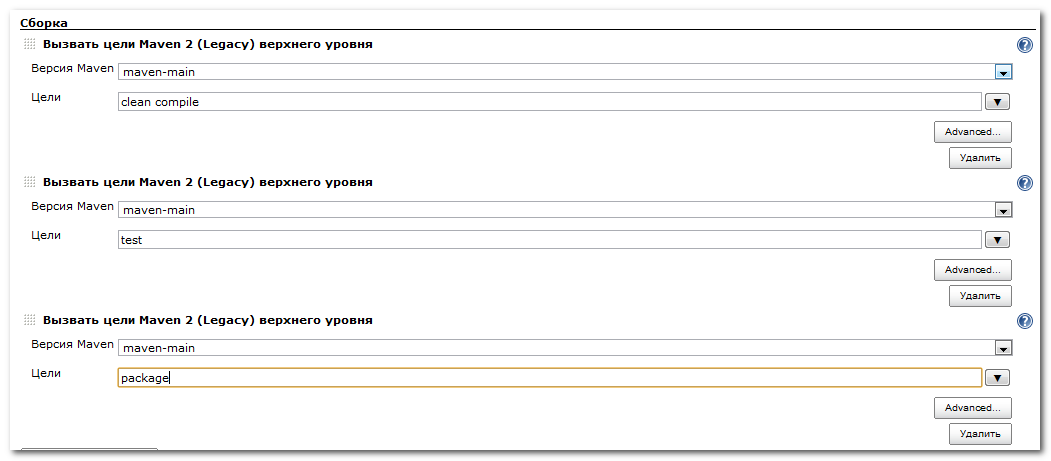
\includegraphics[scale = 0.6]{new-job-5.png}
  \vspace{-10pt}
  \caption{Шаги сборки}
  \label{pic.hudson.job.steps}
\end{center}
\end{figure}

После этого в пункте `\texttt{Послесборочные операции}'' отметить ``\texttt{Publish JUnit test result report}'' и в поле
``\texttt{XML файлы с отчетами о тестировании}'' указать где будут находится \texttt{*.xml} файлы, сгенерированные JUnit. 
По умолчанию maven-плагин \texttt{surefire} помещает эти файлы в директорию
``\texttt{<project-name>/target/surefire-reports}''.
Так как в pom.xml явно не прописано иное, указываем ``\texttt{target/surefire-reports/*.xml}'' (см. рис.
\ref{pic.hudson.job.after-build}).

\begin{figure}[htp]
\begin{center}
  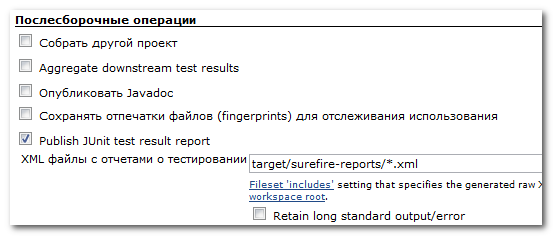
\includegraphics[scale = 0.6]{new-job-6.png}
  \vspace{-10pt}
  \caption{Послесборочные операции}
  \label{pic.hudson.job.after-build}
\end{center}
\end{figure}

Далее нажимаем на кнопку ``\texttt{Сохранить}'' и на этом конфигурация задачи завершена. 

\subsection{Работа с Hudson}

После созадния задачи Hudson выкачает исходные коды и попытается выполнить шаги сборки, которые были указаны при
конфигурации задачи.

На главной странице появилась индикация работы Hudson над отдельными проектами (см. рис. \ref{pic.hudson.start-page}).

\begin{figure}[htp]
\begin{center}
  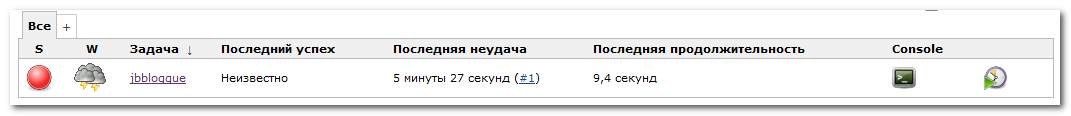
\includegraphics[scale = 0.65]{job-1.png}
  \vspace{-20pt}
  \caption{Стартовая страница Hudson}
  \label{pic.hudson.start-page}
\end{center}
\end{figure}

Если перейти в задачу ``\texttt{jbbloggue}'', которая была создана в подразделе \ref{sec.job-createion}, то а боковой
паели можно увидеть панель ``\texttt{История сборок}'' (см. рис. \ref{pic.hudson.build-history}). В данном случае сборка
упала. Чтобы посмотреть ошибки можно перейти в сборку (кликнув, в данном случае, на время сборки  --
``\texttt{01.05.2012 16:45:52}'') и на боковой панели нажать на ссылку ``\texttt{Вывод консоли}'' (см. рис.
\ref{pic.hudson.build-sidebar}).

\begin{figure}[htp]
	\begin{minipage}[h]{0.49\linewidth}
		\begin{center}
			  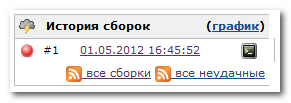
\includegraphics[scale = 0.8]{job-2.png}
			  \vspace{-15pt}
			  \caption{Панель ``История сборок''}
			  \label{pic.hudson.build-history}
		\end{center}
	\end{minipage}
	\hfill
	\begin{minipage}[h]{0.49\linewidth}
		\begin{center}
		  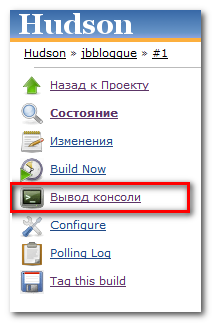
\includegraphics[scale = 0.8]{job-3.png}
		  \vspace{-15pt}
		  \caption[labelInTOC]{Боковая панель сборок}
		  \label{pic.hudson.build-sidebar}
		\end{center}
	\end{minipage}
\end{figure}

В данном случае ошибка заключалась в отсутствии дескриптора развертывания (см. рис. \ref{pic.hudson.console})

\begin{figure}[htp]
\begin{center}
  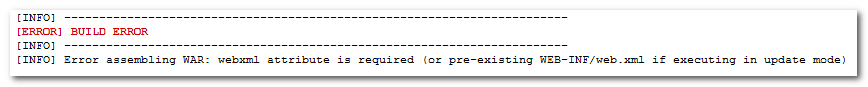
\includegraphics[scale = 0.7]{job-4.png}
  \caption[labelInTOC]{Боковая панель сборок}
  \label{pic.hudson.console}
\end{center}
\end{figure}

Исправляем ошибку и фиксируем изменения в репозитории. После фиксации Hudson выкачает свежую версию проекта и удачно
соберет его (см. рис. \ref{pic.hudson.build-successful}).

\begin{figure}[htp]
\begin{center}
  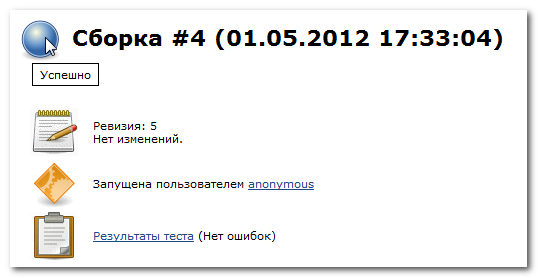
\includegraphics[scale = 0.6]{job-5.png}
  \caption[labelInTOC]{Удачная сборка проекта}
  \label{pic.hudson.build-successful}
\end{center}
\end{figure}


На странице сборки также можно посмотреть результаты запуска тестов. Для этого нужно перейти на страницу
``\texttt{Результаты теста}'' (см. рис. \ref{pic.hudson.test}).

\begin{figure}[htp]
\begin{center}
  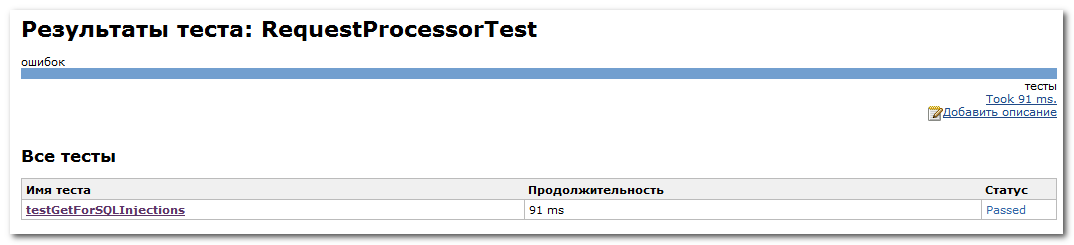
\includegraphics[scale = 0.6]{job-6.png}
  \caption[labelInTOC]{Просмотр результатов тестирования}
  \label{pic.hudson.test}
\end{center}
\end{figure}
\subsection{Дополнительно}
Также Hudson есть возможность подключать дополнительные плагины, например, для инспекции кода.
Наиболее популярные плагины:
\begin{enumerate}
  \item \href{http://findbugs.sourceforge.net/}{FindBugs}; 
  \item \href{http://wiki.hudson-ci.org/display/HUDSON/DRY+Plugin}{DRY-plugin} 
  \item \href{http://wiki.hudson-ci.org/display/HUDSON/Checkstyle+Plugin}{Checkstyle Plug-in}
  \item \href{https://www.atlassian.com/software/clover/overview}{Clover plugin}
\end{enumerate}

\end{document}
